\section{Node Collapse}
In a parallel DAG task, one approach to introduce inter-thread cache benefit is to execute nodes with the same code segment/executable object on the same core. This approach allows the second node to re-use cache blocks loaded into the cache by the first node. In this paper, we focus on this approach of obtaining inter-thread cache benefit, i.e., executing nodes with same code segment on the same core. 

To enable execution of two nodes on the same core, we introduce the concept of collapse of nodes in a DAG. Two nodes $u,v$ of the DAG $G_i$ that have the same code segment can be collapsed into one node $\hat{u}$. We refer to $\hat{u}$ as the collapsed node. Such a collapse also results in a new DAG representation $\hat{G_i} = (\hat{V_i}, \hat{E_i})$ of the same task $\tau_i$.  We refer to the new DAG representation $\hat{G_I}$ as the collapsed DAG. The exact changes to the 

 The collapsed node $\hat{u}$ is represented as a tuple $\hat{u} = \langle \alpha_u , c_u(\eta_{\hat{u}}), \eta_{\hat{u}} \rangle$. The collapsed node will represent the execution
  
 \begin{definition}{Collapse}
Two nodes $u,v \in V_i$ of a DAG $G_i$ are collapsed into one node $\hat{u} \in \hat{V_i}$ to generate a collapsed DAG $\hat{G_i}$, which represents the same task $\tau_i$. The collapsed node $\hat{u}$ is expressed as $\hat{u} = \langle \alpha_u , c_u(\eta_w), \eta_{\hat{u}} = \eta_u+\eta_v \rangle$. The collapsed DAG $\hat{G_i} = (\hat{V_i}, \hat{E_i})$ adheres to the following properties
\begin{itemize}
\item $\exists x \prec^{1} \hat{u}$ in $\hat{G_i}$ $\forall x \prec^1 v$ in $G_i$; i.e., all parent node dependencies of $v$ are preserved in the collapsed DAG.
\item $\exists \hat{u} \prec^{1} y$ in $\hat{G_i}$ $\forall v \prec^1 y$ in $G_i$; i.e., all child node dependencies of $v$ are preserved in the collapsed DAG.
\end{itemize}
 \end{definition}

The collapsed node $\hat{u}$ represents the execution of $\eta_{\hat{u}}$ threads on the code segment of $u$, where $\eta_{\hat{u}} = \eta_u+\eta_v$. The worst case execution time of the collapsed node $\hat{u}$ can be obtained as function of the $\eta_{\hat{u}}$. The collapsed node $\hat{u}$ can be represented as a tuple $\hat{u} = \langle \alpha_u , c_u(\eta_{\hat{u}}), \eta_{\hat{u}} \rangle$. To maintain the parent and child dependencies of the original DAG $G_i$, we replace all edges $(x , v) , (v, y) \forall x, y$ with edges $(x, u), (u, y)$. Note that, collapsing $u$ into $v$ is the same as collapsing $v$ into $u$. For the sake of simplicity in understanding, we collapse node that is not on the critical path into the node on the critical path. For example, if $u$ is on the critical path and has the same code segment as node $v$, then we collapse $v$ into $u$, i.e., the collapsed node is given as $\hat{u} =  \langle \alpha_u , c_u(\eta_{\hat{u}}), \eta_{\hat{u}} \rangle$.


\begin{figure}
  \centering
  \begin{subfigure}[b]{0.4\textwidth}{
      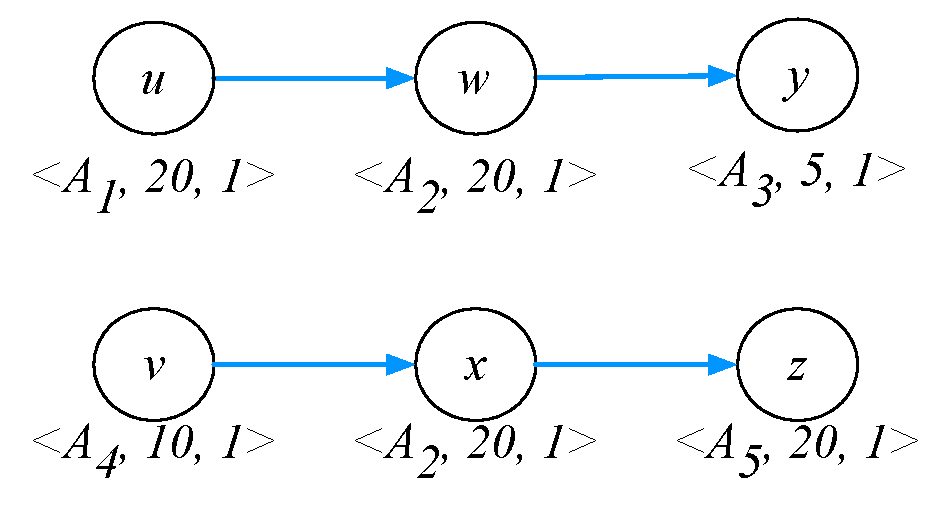
\includegraphics[width=\textwidth]{beforeCollapse}
      \caption{Before Collapse}
      \label{fig:before-collapse}
    }
  \end{subfigure} \quad
  \begin{subfigure}[b]{0.4\textwidth}{
      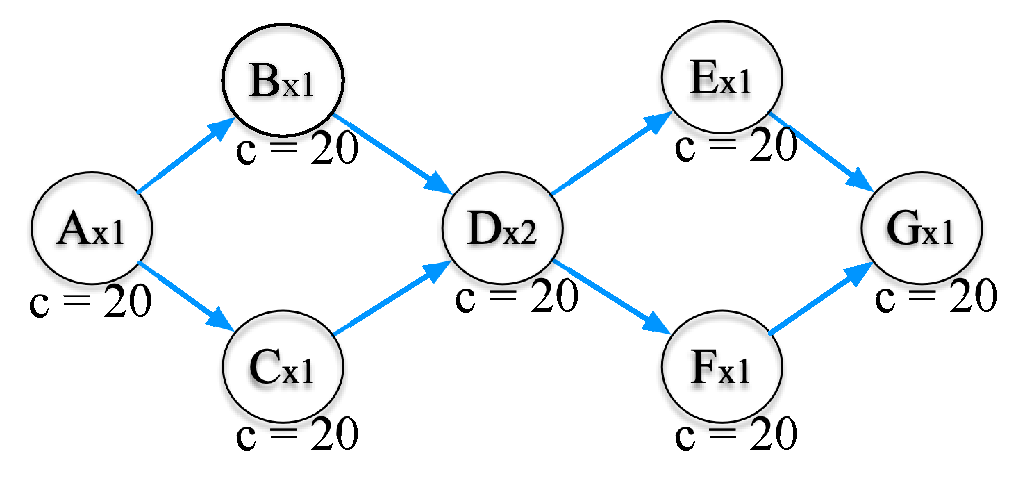
\includegraphics[width=\textwidth]{afterCollapse}
      \caption{After Collapse}
      \label{fig:after-collapse}
    }
  \end{subfigure}
  \caption{An example showing collapse of two nodes}
  \label{fig:dag-collapse}
\end{figure}

Fig.~\ref{fig:dag-collapse} illustrates the collapse of two nodes. Nodes in
Fig.~\ref{fig:before-collapse} are labeled with their node ID and show the tuple representation of the code segment, worst case execution time and number of threads executing the node. Nodes $w$ and $x$ are executing one thread each over the same code segment $A_2$ with worst case execution time 20 units. These two nodes can be collapsed into a single node $t$ with two threads of execution over code segment $A_2$. Assuming that $A_2$ can fit into the cache and the ratio of memory demand to execution demand is$10:1$, the worst case execution time of $t$ can be computed to be $22$, as shown in
Fig.~\ref{fig:after-collapse}.

%% \revise{A property of collapse must be stated. When collapsing two
%%   nodes ${u,v \in V}$ to one node ${u}$ the length of the critical
%%   path is reduced by the WCET of ${v}$ before collapse and increased
%%   by the WCET of ${u}$ after collapse}
  





\section{Candidacy for collapse}
As discussed in the previous section, collapsing two nodes in the DAG can result in an inter-thread cache benefit. However, in some cases, collapsing two nodes may not result in any inter-thread cache benefit. In this section, we define candidates for collapse as a pair of nodes which when collapsed have the potential only to introduce inter-thread cache benefit. 

For a task ${\tau_i \in \tau}$, associated DAG ${G_i \in \mathbb{G}}$,
where ${G_i = (V, E)}$, the nodes ${u,v \in V}$ qualify as
\emph{candidates} for collapse if and only if the following conditions
are true: 
\begin{enumerate}
  \item Nodes ${u}$ and ${v}$ refer to execution of the same object.
  \item Collapsing ${u}$ and ${v}$ cannot not introduce a cycle in ${G_i}$.
  \item The sum of the individual worst-case execution times of ${u}$
    and ${v}$ is greater than the collapsed worst-case execution time
    of ${u}$ and ${v}$ i.e. ${c(\eta_u) + c(\eta_v) > c(\eta_u + \eta_v)}$.
\end{enumerate}

One straightforward property of candidacy is that the nodes $u$ and $v$ should represent the execution over the same code segment.  If the code-segments are different, it can introduce more delays due to context switches between the two threads and cache block evictions. 

Another property of candidacy is that execution of two thread on the same core should be less sequential execution of both the blocks, i.e., ${c(\eta_u) + c(\eta_v) > c(\eta_u + \eta_v)}$. 

\begin{figure}
  \centering
  \begin{subfigure}[b]{0.48\textwidth}{
      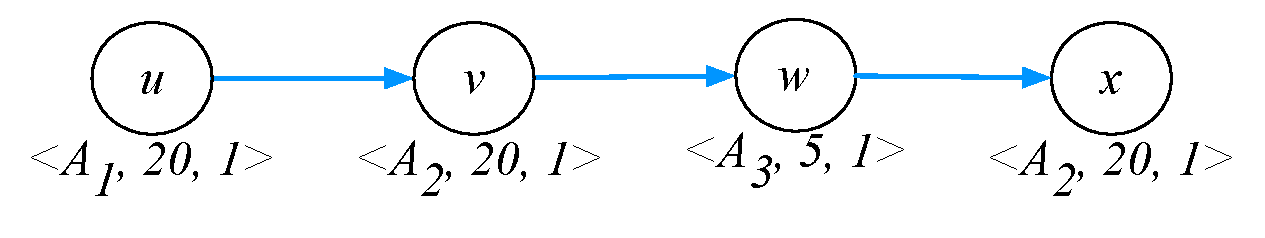
\includegraphics[width=\textwidth]{beforeViolation}
      \caption{Before Collapse}
      \label{fig:beforeViolation}
    }
  \end{subfigure}~
  \begin{subfigure}[b]{0.33\textwidth}{
      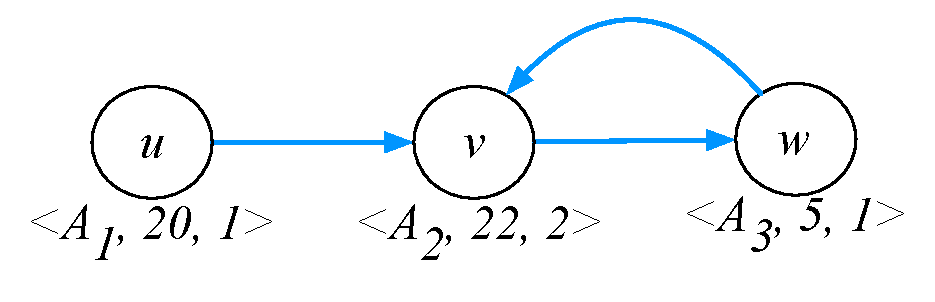
\includegraphics[width=\textwidth]{afterViolation}
      \caption{After Collapse}
      \label{fig:afterViolation}
    }
  \end{subfigure}
  \caption{Collapse of two nodes can result in a loop inside the DAG task}
  \label{fig:dag-violation}
\end{figure}


Finally, the third property of candidacy is that when two nodes are collapsed, it should not introduce any loops in the DAG. For example, Fig~\ref{fig:dag-violation} shows one such example where collapsing two nodes with the same code segment $B$ results in a loop inside the DAG. If the collapse of two nodes introduces a loop, then the scheduler cannot break out of the loop and will execute the nodes in the loop forever. Here, we derive the necessary and sufficient condition for a pair of nodes to not introduce a loop when collapsed.

\revise{Needed: introductory paragraph to state the following theorem
  provides a condition for ensuring collapse does not introduce loops}



\textbf{Definition ${d(u, v)}$} -- is the greatest number of edges
along a directed path from ${u}$ to ${v}$ in ${G}$. When no path
exists, ${d(u,v) = 0}$.

\begin{theorem}[Candidacy for Collapse]
  For a DAG ${G = (V, E)}$ and nodes ${u, v \in V}$ where ${u \prec
    v}$, ${u}$ and ${v}$ can be collapsed without introducing a loop
  if and  only if ${d(u, v) \le 1}$.
\end{theorem}


\begin{theorem}[Candidacy for collapse] \label{thrm:candidacy-collapse} Two nodes $v_i^j$ and $v_i^k$ in a DAG task $\tau_i$ when collapsed do not introduce a loop if and only if $d(v_i^j, v_i^k) \le 1$ and $d(v_i^k, v_i^j) \le 1$, where $d(v_i^j, v_i^k)$ is the length of the longest path between $v_i^j$ and $v_i^k$ as obtained by depth first search. \end{theorem}
\begin{proof}
%The proof is divided into two parts
We divide the proof into two parts. We first prove that the condition $d(v_i^j, v_i^k) \le 1$ and $d(v_i^k, v_i^j) \le 1$ is a necessary condition for candidacy and latter we prove that the condition is a sufficient condition.

%First part - necessary part - to prove that if the constraint is violated then it will result a violation of the dag 
If the condition is not satisfied $d(v_i^j, v_i^k) \le 1$ and $d(v_i^k, v_i^j) \le 1$, then it implies that there is a path from $v_i^j$ to $v_i^k$ or a path from $v_i^k$ and $v_i^j$ with length greater than 1, i.e., $\exists p1 \  such \  that p1 = {v_i^j, v_i^l, \cdots , v_i^k} or p1 = {v_i^k, v_i^l, \cdots , v_i^l}$. When nodes $v_i^j$ and $v_i^k$ are collapsed into $v_i^h$, $p1$ will be modified to ${v_i^h, v_i^l, \cdots , v_i^h}$ which forms a loop. 

%Second part -  sufficient part - if the constraint is met there is no other source of a loop
To prove the sufficient condition, we first prove the contra-positive to be true, i.e., a DAG violation occurs only when the condition $d(v_i^j, v_i^k) \le 1$ and $d(v_i^k, v_i^j) \le 1$ is true. A DAG violation in the collapsed DAG implies that there exists a path $p1$ in the collapsed DAG given by $v_i^h, v_i^l, \cdots , v_i^h$ with a length greater than or equal to 2.  Since there are no loops in the original DAG, only a collapsed node can cause a loop in the collapsed DAG. Therefore, $v_i^h$ should be the collapsed node. In the original DAG, one node of $v_i^h$ corresponds to $v_i^j$ and the other node corresponds to $v_i^k$. In the original DAG, $p1$ must correspond to ${v_i^j, v_i^l, \cdots , v_i^k} or {v_i^k, v_i^l, \cdots , v_i^l}$. Thus, a DAG violation in the collapsed DAG implies that there exists a path from $v_i^j$ to $v_i^k$  or $v_i^k$ and $v_i^j$ with a length greater than or equal to 2. 

Therefore, we can conclude that two nodes $v_i^j$ and $v_i^k$ in a DAG task $\tau_i$ when collapsed do not introduce a loop if and only if $d(v_i^j, v_i^k) \le 1$ and $d(v_i^k, v_i^j) \le 1$.
\end{proof}

In summary, we define two nodes $v_i^j$ and $v_i^k$ to be {\textbf candidates for collapse} if they have the same code block and $d(v_i^j, v_i^k) \le 1$ and $d(v_i^k, v_i^j) \le 1$, where $d(v_i^j, v_i^k)$ is the length of the longest path between $v_i^j$ and $v_i^k$.
